\chapter{Устройство приложения}
	Серверная часть данного проекта состоит из внешнего сервера, внутренних серверов и базы данных, см рис.\ref{fig:app_schema}.
\begin{figure}[h]
	\begin{center}
	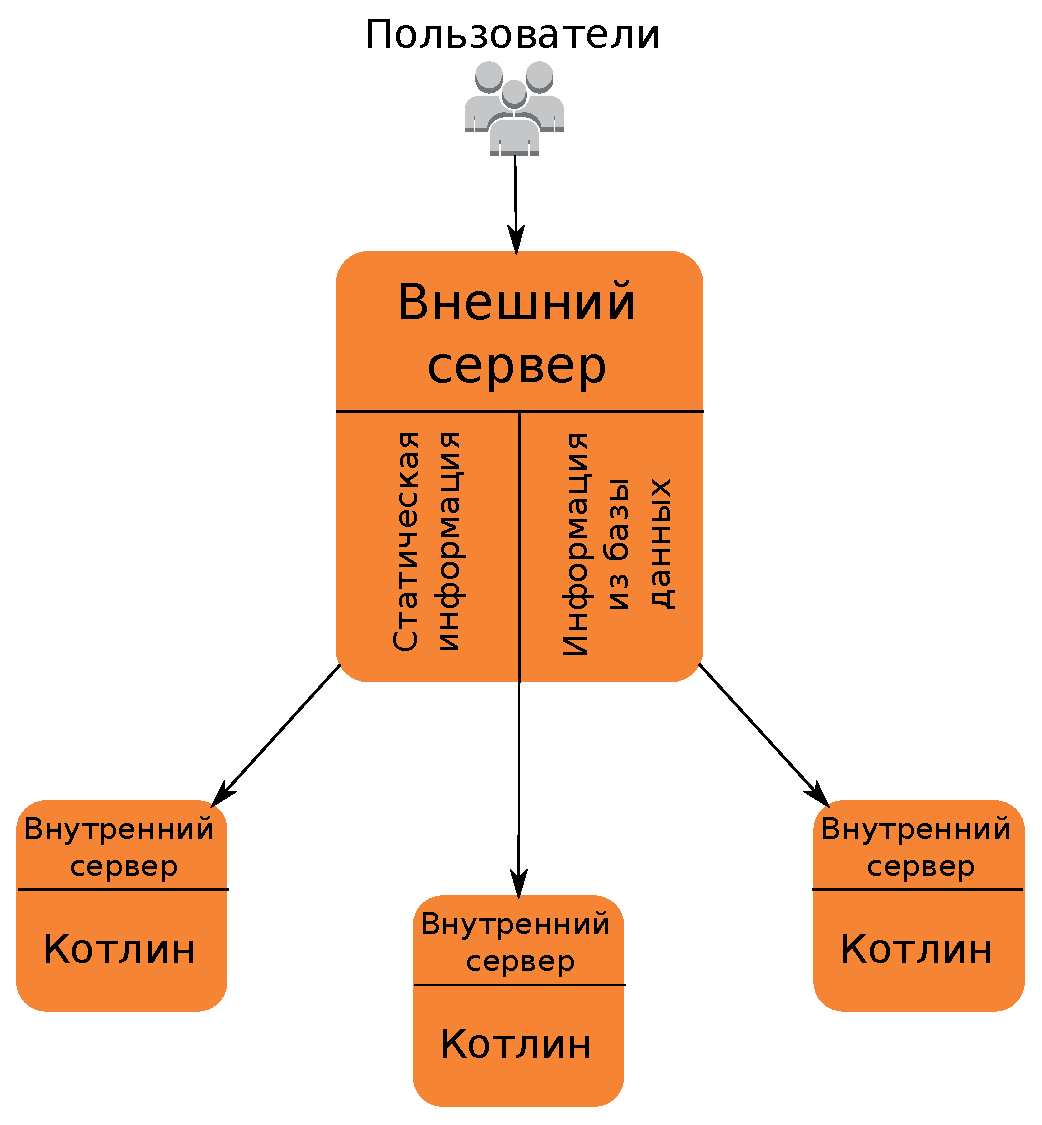
\includegraphics[scale=0.8]{app_schema}
	\end{center}
	\caption{Устройство серверной части приложения}
	\label{fig:app_schema}
\end{figure}	


\section{База данных}
	В данном проекте используются две базы данных, схемы которых приведены в приложении. Обе базы используются исключительно внешним сервером.
	
	Первая база данных~--- это база данных приложения, в ней хранится информация о пользовательских проектах. Данная база состоит из трёх таблиц~--- таблицы с пользователями, таблицы с проектами и таблицы с файлами. Каждый проект имеет ссылку на автора, каждый файл имеет ссылку на проект, к которому он принадлежит. 
Во всех трёх таблицах помимо первичных ключей, которые используются только внутри базы, имеются дополнительные ключи, которые используются в HTTP-запросах.
	
	Вторая база данных используется внешним сервером для хранения информации о HTTP-сессиях. Такой подход к хранению сессий позволяет разделять эту информацию между различными серверами и, благодаря этому, не терять её при обновлении приложения. 

	
	%Написать про базу данных
	%Добавить картинку
	%Обновление бэкенда при обновлении версии Котлина
	%Сказать про JS конфигурацию
\section{Внешний сервер}
	Внешний сервер принимает все запросы, приходящие от пользователя. Эти запросы делятся на несколько типов:
\begin{itemize}
	\item Запросы, обрабатываемые на внешнем сервере
	\item Запросы  к базе данных
	\item Запросы к внутренним серверам
\end{itemize}

	На внешнем сервере, в основном, обрабатываются запросы на получение статических данных. К этим данным, в первую очередь, относится вся клиентская часть кода в виде HTML/CSS/JavaScript файлов. Также к статическим данным относятся примеры, хранящиеся на внешнем сервере.
	
	%TODO: проверка синтаксиса считает, что можно "авторизоваться", но не "авторизироваться". Поправь ранее
	%TODO: Авторизоваться = залогинться = войти в свою учётную запись = войти в свой профиль, сделай что-нибудь с этим адом лексических повторов
	Кроме запросов на получение статических данных, внешний сервер обрабатывает запросы на авторизацию. Поскольку в данном приложении отсутствует встроенный механизм авторизации, то все эти запросы перенаправляются на сайт другого сервиса, позволяющего пользователю авторизоваться. Если авторизация прошла успешно, то сервис авторизации возвращает всю интересующую нас информацию, в нашем случае~--- идентификатор пользователя и его имя. На данный момент авторизоваться можно через сервисы google, facebook, twitter, github или JetBrainsAccount. Во всех случаях, кроме сервиса JetBrainsAccount, для авторизации используется протокол OAuth.
	
	
	При успешной авторизации информация о пользователе записывается в HTTP-сессию и, если пользователь заходит впервые, заносится в базу данных.
	
	
	Запросы к базе данных отправляются только для авторизованных пользователей. Данные запросы позволяют выполнять все необходимые операции с пользовательскими проектами и файлами (получить, создать, обновить, удалить).
	
	%TODO: проверь, что все "в течении" -> "в течение". Т.к. ты работаешь с промежутками времени, а не с рекой воды
	Все запросы, связанные с Котлином, пересылаются внутренним серверам, после чего в течение определённого времени ожидается ответ, который отправляется обратно пользователю. Если же ответ не приходит, то пользователю отправляется соответствующее сообщение об ошибке.
	
	

\section{Внутренний сервер}
	Как уже было сказано в предыдущей главе, внутренний
сервер обрабатывает запросы, связанные с Котлином. Эти запросы делятся на 5 типов:
\begin{itemize}
	\item Запросы на получение списка ошибок в коде
	\item Запросы на автодополнение
	\item Запросы на конвертацию кода на языке Java в код на языке Котлин
	\item Запросы на трансляцию кода на языке  Котлин в код на языке Java\-Script.
	\item Запросы на исполнение кода на языке Котлин.
\end{itemize}
	Для обработки этих запросов на внутреннем сервере используется последняя версия библиотек Котлина. Обработка всех запросов, кроме запросов на исполнение программ, в итоге сводится к вызову методов из этих библиотек. Такой подход является наиболее простым, однако у него есть один недостаток~--- мы не можем ограничить время исполнения вызванного метода, а значит и время обработки запроса. Это связано с тем, что поток в языке Java не может быть завершён извне. 
	
	%TODO: любишь писать "и.т.д." вместо "и т.д."
	При обработке запроса на исполнение сначала, при помощи библиотек Котлина, код компилируется в байткод JVM. Далее скомпилированный код исполняется в отдельном процессе внутри класса-обёртки. В целях безопасности	процесс, в котором исполняется пользовательская программа, ограничен по памяти (Xmx настройка java-машины), ограничен по времени исполнения (через 5 секунд процесс завершается из сервера), а также ему запрещён доступ к сети, файловой системе и т.д. при помощи Java security manager(см. рис.\ref{fig:backend_schema}).
	
\begin{figure}[ht]
	\begin{center}
		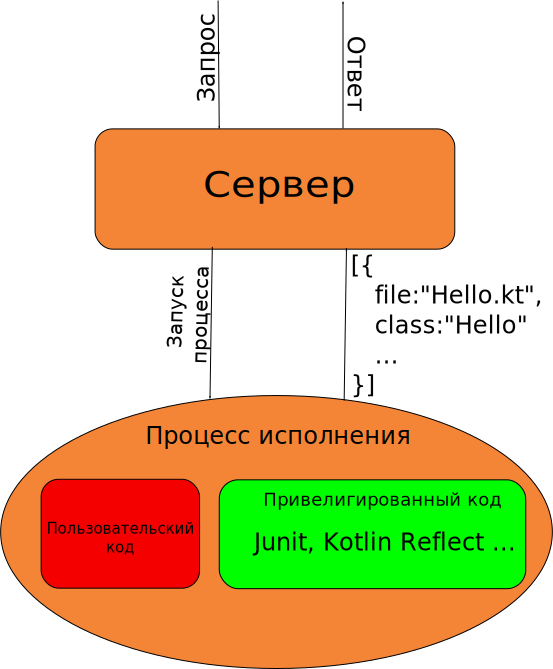
\includegraphics[scale=0.6]{backend_schema.eps}
	\end{center}
	\caption{ Схема запуска пользовательского когда на внутреннем сервере}
	\label{fig:backend_schema}
\end{figure}
	
	В случае JVM конфигурации класс-обёртка, используя reflection, запускает функцию main в пользовательском коде, то есть просто исполняет пользовательскую программу. При этом весь вывод программы (System.out,  Sys\-tem.err) перенаправляется в форматированном виде в один поток. Если внутри пользовательского кода происходит исключение, то оно ловится классом-обёрткой. По завершении пользовательской программы весь вывод, а также исключение (если есть), сериализуются в формат JSON(см. листинг \ref{lst:output_example}) и полученная строчка выводится в стандартный вывод класса-обёртки.
	
\begin{lstlisting}[caption=Пример вывода программы в случае JVM конфигурации, label=lst:output_example]
{
  "text":"<outStream>Hello, world!\n</outStream>;",
  "exception":		
  {
    "message":null,
    "fullName":"java.lang.Exception",
    "stackTrace":
    [
      {
        "methodName":"main",
        "fileName":"Simplest version.kt",
        "lineNumber":8,
        "className":"_DefaultPackage$Simplest version$f7f9443d",
	 			"nativeMethod":false
      },
      {
        "methodName":"main",
        "fileName":"Simplest version.kt",
        "lineNumber":1,
        "className":"_DefaultPackage",
        "nativeMethod":false
      }
    ],
    "cause":null
}
}
\end{lstlisting}
	
	%TODO: "по завершению" -> "по завершении" исправь, где найдёшь ещё.
	В случае Junit конфигурации запускаются все тестовые методы, найденные внутри пользовательских классов. При запуске каждого теста сохраняется вывод программы и ошибки, произошедшие в процессе исполнения. По завершении исполнения всех тестов эта информация так же сериализуется в формат JSON и выводится в стандартный поток вывода.
	

	
	
	